\subsection{Migration}
Bei der Verwendung mehrerer Subpopulationen entwickeln sich diese zunächst 
unabhängig voneinander. Um nun aber auch global von den lokal in den 
Subpopulationen entstandenen Individuen profitieren zu können, wird nach 
einiger Zeit Information zwischen den einzelnen Populationen ausgetauscht - 
dies geschieht durch den Austausch einzelner Individuen. Diesen Vorgang nennt 
man \textsl{Migration}. Nach dem Austausch von Individuen entwickeln sich die 
Populationen wieder eine Zeit lang unabhängig voneinander, bis der 
Austauschvorgang von neuem beginnt \cite{url:geatbx-documentation}.

Der Parameter \texttt{Topology} legt fest, welche Topologie bei der Migration 
verwendet wird. Unter Topologie ist in diesem Zusammenhang zu verstehen, 
\textsl{welche} Unterpopulationen Individuen untereinander austauschen. Dieser 
Parameter kann in der GEATbx die folgenden drei Werte annehmen:

\begin{itemize}
  \item 0: Vollständige Netzstruktur ohne Einschränkungen, d.h. Individuen 
  können zwischen \textsl{allen} Subopulationen ausgetauscht werden.
  \item 2: Ringstruktur, d.h. die Subpopulationen werden ringförmig angeordnet 
  und Individuen können nur in die im Ring folgende Subpopulation migrieren.
  \item 1: Nachbarschaftsstruktur, ähnlich zur Ringstruktur. Jedoch können 
  Individuen in beiden Richtungen zwischen den Nachbarn transferiert werden.
\end{itemize}

Der Parameter \texttt{Rate} bestimmt, welcher Anteil jeder Population bei der 
Migration migriert werden soll. Dabei können Werte im Bereich von $[0, 1]$ 
angegeben werden. Die Werte repräsentieren prozentuale Angaben; so sorgt also 
z.B. das Setzen des Parameters auf den Wert 0.20 dafür, dass 20\% der 
Individuen bei der Migration ausgetauscht werden. Mittels des Parameters 
\texttt{Interval} lässt sich einstellen, wie oft (d.h. nach welcher Anzahl von 
Generationen) eine Migration stattfinden soll.

\subsection{Testläufe mit variierenden Populationsgrößen}
\label{subsec:TestlaeufePopulationsgroessen}
Für die Durchführung dieser Testreihe wurde das bereits beschriebene Skript 
verwendet; variiert wurden die folgenden Parameter:

\begin{description}
  \item[Subpopulationen:] 1, 5, 8 und 12.
  \item[Individuen pro Population:] 15, 30, 45, 60.
\end{description}

Für die 16 möglichen Kombinationen wurden jeweils 20 Testläufe durchgeführt und
am Ende der Mittelwert berechnet. Insgesamt umfasste die Testreihe demnach 320
Testläufe. Die Anzahl der Generationen war hierbei stets auf 100 fixiert.

Die Ergebnisse der Testläufe sind in Tabelle \ref{tbl:aufgabeC-ergebnisse}
aufgeführt. 

\begin{table}
	\sffamily
	\centering
	\footnotesize
	\begin{tabularx}{\textwidth}{NXlllll}
		\toprule
		\multicolumn{1}{@{}N}{Nr.} &
		\multicolumn{1}{V{3.5em}@{}}{Subpop.} &
		\multicolumn{1}{V{3.5em}@{}}{Indiv.} &
		\multicolumn{1}{V{5em}@{}}{Mittelwert $\bar{x}$} &
		\multicolumn{1}{V{6.5em}@{}}{Standardabw. $\sigma_x$} &
		\multicolumn{1}{V{9em}@{}}{Minimalwert in Lauf $r$, Generation $g$} &
		\multicolumn{1}{V{9em}@{}}{Maximalwert in Lauf $r$, Generation $g$} \\
		\midrule\addlinespace
		1 & 1 & 15 & 3093,30 & 215,63 & 2793, $r = 10$, $g = 95$ & 3715, $r = 20$, $g
		= 95$ \\ \cmidrule(rl){1-7}
		2 & 5 & 15 & 2693,55 & 128,33 & 2443, $r = 12$, $g = 97$ & 2889, $r = 11$, $g
		= 94$ \\ \cmidrule(lr){1-7}
		3 & 8 & 15 & 2644,65 & 136,63 & 2361, $r = 15$, $g = 94$ & 2904, $r = 16$, $g = 99$ \\ \cmidrule(lr){1-7}
		4 & 12 & 15 & 2521,25 & 91,48 & 2269, $r = 16$, $g = 91$ & 2662, $r = 14$, $g = 97$ \\
		\midrule
		5 & 1 & 30 & 3024,40 & 243,43 & 2719, $r = 5$, $g = 89$ & 3567, $r = 18$, $g = 100$ \\ \cmidrule(lr){1-7}
		6 & 5 & 30 & 2464,70 & 119,89 & 2253, $r = 2$, $g = 88$ & 2857, $r = 7$, $g = 97$ \\ \cmidrule(lr){1-7}
		7 & 8 & 30 & 2448,15 & 112,17 & 2192, $r = 3$, $g = 99$ & 2622, $r = 7$, $g = 87$ \\ \cmidrule(lr){1-7}
		8 & 12 & 30 & 2416,70 & 103,81 & 2209, $r = 5$, $g = 96$ & 2564, $r = 9$, $g = 95$ \\
		\midrule
		9 & 1 & 45 & 2838,25 & 213,74 & 2493, $r = 6$, $g = 91$ & 3153, $r = 17$, $g = 83$ \\ \cmidrule(lr){1-7}
		10 & 5 & 45 & 2378,00 & 117,79 & 2173, $r = 15$, $g = 100$ & 2632, $r = 3$, $g = 99$ \\ \cmidrule(lr){1-7}
		11 & 8 & 45 & 2347,50 & 105,99 & 2189, $r = 11$, $g = 99$ & 2610, $r = 14$, $g = 96$ \\ \cmidrule(lr){1-7}
		12 & 12 & 45 & 2309,85 & 98,98 & 2168, $r = 9$, $g = 99$ & 2497, $r = 17$, $g = 90$ \\
		\midrule
		13 & 1 & 60 & 2747,60 & 157,29 & 2395, $r = 16$, $g = 100$ & 3071, $r = 8$, $g = 99$ \\ \cmidrule(lr){1-7}
		14 & 5 & 60 & 2386,35 & 101,48 & 2157, $r = 19$, $g = 96$ & 2558, $r = 8$, $g = 98$ \\ \cmidrule(lr){1-7}
		15 & 8 & 60 & 2320,75 & 105,88 & 2143, $r = 4$, $g = 97$ & 2540, $r = 18$, $g = 99$ \\ \cmidrule(lr){1-7}
		16 & 12 & 60 & \textbf{2285,85} & 88,91 & \textbf{2115}, $r = 20$, $g = 90$ & 2422, $r = 8$, $g = 96$ \\

		\addlinespace\bottomrule
		\end{tabularx}
	\caption{Ergebnisse der Testreihe}
	\label{tbl:aufgabeC-ergebnisse}
\end{table}

\subsubsection{Interpretation der Ergebnisse}
Wie man an den Testergebnissen sieht, erhöht sich die Güte des Resultats sowohl
mit der Anzahl der \textsl{Subpopulationen} als auch der \textsl{Individuen pro
Population}. Innerhalb der Testläufe mit gleicher Individuenanzahl verbessert
sich der Mittelwert deutlich mit steigender Subpopulationsanzahl. Und auch
zwischen den Testfällen mit steigender Individuenanzahl ist erkennbar, dass die
Ergebnismittelwerte besser sind. Abbildung \ref{fig:aufgabeC-plot} zeigt eine
grafische Auswertung der Testergebnisse.

\begin{figure}
  \centering
  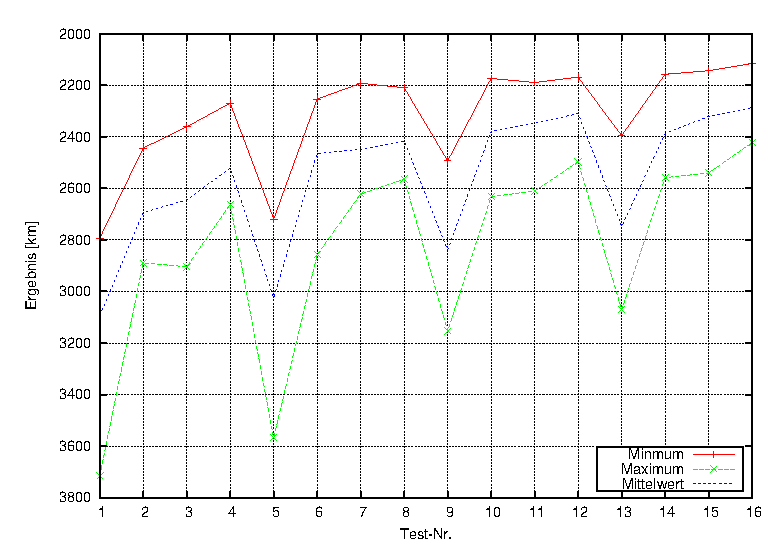
\includegraphics[width=1.0\textwidth]{../images/aufgabeC-plot}
  \caption{Grafische Darstellung der Testreihe: Minimal-, Maximal- und
  Mittelwert}
  \label{fig:aufgabeC-plot}
\end{figure}

Das beste Testergebnis von 2115 km (in der Tabelle fett markiert) erhielten wir
erwartungsgemäß bei den jeweiligen Maximalwerten der variierten Parameter.